\documentclass[preprint,12pt,a4paper]{elsarticle}
\usepackage{lineno}
\usepackage{hyperref}
\usepackage{float}
\usepackage{graphicx} % figuras
% \usepackage{subfig}
\usepackage{subfigure} % subfiguras
\usepackage{multirow} 
\usepackage{color}
\usepackage{soul}
\usepackage{cancel}

%%%%%%%%%%%%%%%%%%%%%%%%%%%%%%%%%%%%%%%%%%%%%%%%%%%%%%%%%%%%%%%%%%%%
% Init macros math

\usepackage[fleqn,tbtags]{amsmath}
\usepackage{mathtools}
\usepackage{amsthm,amssymb}
\usepackage{xstring}

\newcommand{\vect}[1]{
  \ensuremath{\mathbf{{#1}}}
}
\newcommand{\tens}[1]{
  \ensuremath{\mathbf{{#1}}}
}
\newcommand{\Matrix}[1]{
  \ensuremath{\mathbf{{#1}}}
}
\newcommand{\Vector}[1]{
  \ensuremath{\mathbf{{#1}}}
}
% Divergence
\newcommand{\Div}[1]{
  \ensuremath{div({#1})}
}
% Gradient
\newcommand\Grad[1]{grad({#1})}
\newcommand\GradS[1]{grad^s({#1})}
\newcommand\GradT[1]{grad^T({#1})}
% Partial derivative
\newcommand{\Deriv}[3][]{
  \ensuremath{\frac{\partial^{#1}{#2}}{ \partial {#3}^{#1} }}
}
% Integral
\newcommand{\Integral}[2]{
  \IfStrEqCase{#1}{
    {2}{\ensuremath{\int_{\varGamma_d}{#2}\ d\varGamma}}
    {3}{\ensuremath{\int_{\varOmega}{#2}\ d\varOmega}}
  }
}
% End macros math
%%%%%%%%%%%%%%%%%%%%%%%%%%%%%%%%%%%%%%%%%%%%%%%%%%%%%%%%%%%%%%%%%%%%


% \usepackage{algorithm,algcompatible}

\usepackage{blindtext}
\usepackage[linesnumbered,boxed]{algorithm2e}

\SetAlCapSkip{1em}

\SetKwInput{KwInput}{Input}
\SetKwInput{KwOutput}{Output}

% \usepackage[linesnumbered,ruled,vlined]{algorithm2e}
% \algnewcommand\INPUT{\item[\textbf{Input:}]}%
% \algnewcommand\OUTPUT{\item[\textbf{Output:}]}%

%%%%%%%%%%%%%%%%%%%%%%%%%%%%%%%%%%%%%%%%%%%%%%%%%%%%%%%%%%%%%%%%%%%%
% Init glossaries
\usepackage[acronym]{glossaries}

\makeglossaries

\newglossaryentry{domain}
{
  name=$\varOmega$,
  description={Continuum domain}
}

\newglossaryentry{contour}
{
  name=$\partial\varOmega$,
  description={Boundary of the continuum domain $\varOmega$. Also
    defined as $\Gamma$}
}

\newglossaryentry{dirichlet-boundary}
{
  name=$ \Gamma_d$,
  description={Essential or Dirichlet boundary conditions over $\partial\varOmega$}
}

\newglossaryentry{neumann-boundary}
{
  name=$ \Gamma_n$,
  description={Natural or Nemann boundary conditions over $\partial\varOmega$}
}

\newglossaryentry{a}
{
  name=$\vect{a}$,
  description={First order tensor which describes the acceleration field}
}

\newglossaryentry{v}
{
  name=$\vect{v}$,
  description={First order tensor which describes the velocity field}
}

\newglossaryentry{u}
{
  name=$\vect{u}$,
  description={First order tensor which describes the displacement field}
}

\newglossaryentry{x}
{
  name=$\vect{x}$,
  description={First order tensor which describes the global coordinates field}
}

\newglossaryentry{xi}
{
  name=$\vect{\xi}$,
  description={First order tensor which describes the local coordinates field}
}


\newglossaryentry{stress}
{
  name=$\tens{\sigma}$,
  description={Second order tensor which means the Cauchy stress tensor}
}


\newglossaryentry{strain}
{
  name=$\tens{\varepsilon}$,
  description={Second order tensor which means the Cauchy strain tensor}
}

\newglossaryentry{Constitutive}
{
  name=$\tens{D}$,
  description={Four order tensor which means the constitutive response
    of the material}
}

\newglossaryentry{LME-beta}
{
  name=$\beta$,
  description={Regularization or thermalization parameter of the
    LME$_{\beta}$ Pareto set}
}

\newglossaryentry{rho}
{
  name=$\rho$,
  description={Describes the scalar density field}
}

\newglossaryentry{fc}
{
  name=f$_c$,
  description={Compressive strenght}
}

\newglossaryentry{ft}
{
  name=f$_t$,
  description={Tensile strenght}
}

\newglossaryentry{Gf}
{
  name=G$_F$,
  description={Specific fracture energy}
}

\newglossaryentry{E}
{
  name=E,
  description={Elastic modulus}
}

\newglossaryentry{nu}
{
  name=$\nu$,
  description={Poisson ratio}
}

\newacronym{mpm}{MPM}{Material Point Method}
\newacronym{otm}{OTM}{Optimal Transportation Meshfree}
\newacronym{sph}{SPH}{Smoothed Particle Hydrodynamics}
\newacronym{fem}{FEM}{Finite Element Method}
\newacronym{efgm}{EFGM}{Element-Free Galerkin Method}
\newacronym{lme}{LME}{Local Maximum-Entropy}
\newacronym{flip}{FLIP}{Fluid Implicit Particle}
\newacronym{gimp}{GIMP}{Generalized Interpolation Material Point}
\newacronym{igimp}{iGIMP}{Implicit GIMP}
\newacronym{ugimp}{uGIMP}{Uniform GIMP}
\newacronym{ddmp}{DDMP}{Dual Domain Material Point}
\newacronym{ctls}{CTLS}{Conservative Taylor Least Squares}
\newacronym{npc}{NPC}{Newmark Predictor-Corrector}
\newacronym{fe}{FE}{Forward Euler}

% End glossaries
%%%%%%%%%%%%%%%%%%%%%%%%%%%%%%%%%%%%%%%%%%%%%%%%%%%%%%%%%%%%%%%%%%%%

\newcommand{\PNA}[1]{
  \textcolor{red}{{#1}}
}

\newcommand{\MMP}[1]{
  \textcolor{blue}{{#1}}
}

\newcommand{\DM}[1]{
  \textcolor{gree}{{#1}}
}

%%%%%%%%%%%%%%%%%%%%%%%%%%%%%%%%%%%%%%%%%%%%%%%%%%%%%%%%%%%%%%%%%%%%

% \journal{Engineering Fracture Mechanics}
\journal{Computers and Structures}

\modulolinenumbers[5]

%%%%%%%%%%%%%%%%%%%%%%%
%% Elsevier bibliography styles
%%%%%%%%%%%%%%%%%%%%%%%
%% To change the style, put a % in front of the second line of the current style and
%% remove the % from the second line of the style you would like to use.
%%%%%%%%%%%%%%%%%%%%%%%

%% Numbered
%\bibliographystyle{model1-num-names}

%% Numbered without titles
%\bibliographystyle{model1a-num-names}

%% Harvard
%\bibliographystyle{model2-names.bst}\biboptions{authoryear}

%% Vancouver numbered
%\usepackage{numcompress}\bibliographystyle{model3-num-names}

%% Vancouver name/year
%\usepackage{numcompress}\bibliographystyle{model4-names}\biboptions{authoryear}

%% APA style
%\bibliographystyle{model5-names}\biboptions{authoryear}

%% AMA style
%\usepackage{numcompress}\bibliographystyle{model6-num-names}

%% `Elsevier LaTeX' style
\bibliographystyle{elsarticle-num}
%%%%%%%%%%%%%%%%%%%%%%%

\begin{document}

\begin{frontmatter}

\title{LME-MPM applied to quasi-brittle fracture.}

% \title{An enhanced EigenMPM }

%% Group authors per affiliation:
\author{
Miguel Molinos$^a$\footnote{Corresponding author: m.molinos@alumnos.upm.es},
Pedro Navas$^a$\footnote{Corresponding author: p.navas@upm.es},
Diego Manzanal$^a$,
and Manuel Pastor$^a$
 }
 \address{
 $^a$ ETSI Caminos, Canales y Puertos, Universidad Polit\'ectnica de Madrid.\\
 c. Prof. Aranguren 3, 28040 Madrid, Spain
}

\begin{abstract}
  The objective of this work is to introduce an alternative
  technique to address the fracture process of brittle and
  quasi-brittle materials under the \acrfull{mpm} 
  framework. With this purpose the eigensoftening algorithm, developed
  originally for the \acrfull{otm} approximation scheme, is extended
  to the \acrshort{mpm} with the aim of present a suitable alternative
  to the existing fracture algorithms developed for the
  \acrshort{mpm}. The good fitting in the predictions made by the
  eigensoftening algorithm against both analytical and experimental
  results proofs the well performance of the method under challenging
  loads.
\end{abstract}

\begin{keyword}
Quasi brittle fracture \sep Local-\textit{max-ent} approximation \sep
Material Point Method \sep Solid Dynamics
\end{keyword}

\end{frontmatter}

\linenumbers

%%%%%%%%%%%%%%%%%%%%%%%%%%%%%%%%%%%%%%%%%%%%%%%%%%%%%%%%%%%%%%%%%%%%%%%%%
\section{Introduction}
\label{sec:1}
Presence of cracks are a violation of the continuity requirement in
\acrfull{fem}. To overcome it, numerous of numerical
artifacts has been proposed with the aim of reproducing such a
complex behaviour. These techniques vary from employing cohesive
approaches \cite{Barenblatt,Hilleborg_1976}, by adaptively inserting
cohesive elements \cite{Ortiz_1999,Pandolfi_2002,Ruiz_2000} at solid
elements boundaries, or handling arbitrary cracks paths by level set
representation of the fracture surface \cite{Belytschko_03}. The
simulation of fracture propagation in a more accurate and effective
way can be considered as one of the original drivers for developing
novel spatial discretization methods like meshfree techniques. Some
examples of it are the \acrfull{mpm}
\cite{Schreyer_2002,Chen_2002,Nairn_2003,Zhenmao_2005}, the
\acrfull{efgm} \cite{BELYTSCHKO_1995,BELYTSCHKO_2000,Zhuang_2012,Muthu_2013}, the
\acrfull{sph} \cite{Wang_2020,Wang_2019}, the \acrfull{otm} \cite{Li2010,Li_2012,Pandolfi_2013,Li_2015} or Peridynamics
\cite{HA_2011,RABCZUK_2017} among others. \\

Regarding \acrshort{mpm}, fracture can be described numerically in
two ways. One is the ``CRAcks with Material Points (CRAMP)''
\cite{Nairn_2003,Nairn_2006} and consist in to remove the restriction
of the single-valued velocity field close to the crack thorough two or
more sets of nodes. In this method, different labels are assigned to the material points
and nodes to distinguish if they are in the same side of the crack or
not. Under this approach crack surface is described with line segments
in 2D and triangle patches in 3D cases. The chosen criteria for crack
propagation is based on such parameters as energy release rate
analyzed by Tan \& Nairn (2002)\cite{Nairn_2002}, and the stress
intensity factor or the J-integral discussed by Guo \& Nairn
(2004)\cite{Nairn_2004}. The other approach is to introduce failed
material points to describe the crack evolution. In this method, the
formation of failed points describes the nucleation of cracks, and
thereafter its propagation and branching. Consequently, the position
of the crack does not need to be explicitly stated. These represents
significant advantages over the ``CRAMP''. Under this approach, the
prediction of failure evolution is computed with a decohesion model,
which has been discussed by Chen {\it et al.}\cite{Zhenmao_2005} and
Schreyer {\it et al.}\cite{Schreyer_2002}. And has been successfully
employed to simulate the fracture of brittle materials by Chen {\it et
  al.} \cite{Chen_2002,Chen_2003} and Sulsky \& Schreyer
\cite{Sulsky_2004}.\\

Similar to this approach, Schmidt {\it et al.}
\cite{Schmidt_2009} introduced the concept of eigenfracture, where
they approximate the crack set by means of eigen-deformations, wich
enable the material to develop displacement jumps at no cost of local
elastic energy. Later, the eigenerosion approach to brittle facture
was developed by Pandolfi {\it et al.}
\cite{Pandolfi_2012,Pandolfi_2013}. In this technique the erosion of
the material point means that each material point can be either intact or be completely failed or eroded and has no load bearing
capacity. This method has been successfully applied to simulate high
complex phenomena such dynamic fragmentation of metals
\cite{Li_2015}. Recently, Zhang {\it et al.}
\cite{Zhang_EE_2020} adopted the eigenerosion to resolve the dynamic
fracture of brittle materials in the \acrshort{mpm}
framework. Nonetheless, in quasi-brittle materials simulations
performed with this approach exhibit an overestimation of tensile
stress and the strain peaks. And conventional \acrshort{mpm}/\acrshort{gimp} always
faces stress oscillations.\\

To overcome the limitations observed in the EigenMPM
\cite{Zhang_EE_2020}. The present research propose the eigensoftening
algorithm developed by Navas {\it et al.}
\cite{Navas_2017_ES,Navas2018a} for the \acrshort{otm} framework and
engineered for quasi-brittle materials. Inspired in the concept of the
crack band model \cite{Bazant83}, since energy dissipation is thorough
the softened (or failed) volume, it is able to capture the gradual rather than abrupt
dissipation of the fracture energy. Second, to mitigate stress
oscillations the \acrfull{lme} approximation technique
\cite{Arroyo2006} to deal with tensile instabilities, such those that
occurs when particles crosses an element boundary.\\

The paper is structured as follows. First meshfree methodology,
eigenerosion and eigensoftening algorithms are presented in Section
\ref{sec:2}. Then, both approaches are compared and verified by means of
comparisons with analytical and experimental results in Section
\ref{sec:3}. Finally, relevant conclusions are exposed in Section \ref{sec:4}.

%%%%%%%%%%%%%%%%%%%%%%%%%%%%%%%%%%%%%%%%%%%%%%%%%%%%%%%%%%%%%%%%%%%%%%%%%
\section{The meshfree methodology}
\label{sec:2}

The aim of this section is to describe and introduce some special
techniques required to face the fracture problem under the \acrshort{mpm}
framework. In consequence it is structured as follows: first in
\ref{sec:2.1} the \acrfull{npc} algorithm for the \acrshort{mpm}
will be exposed, next the \acrshort{lme} approximants are
introduced in \ref{sec:2.2} as an accurate alternative technique to
interpolate data between particles and nodes, and finally fracture
algorithms based in the eigendeformation concept are presented in \ref{sec:2.3}.

\subsection{The \acrshort{mpm} time integration : A \acrlong{npc}  scheme}
\label{sec:2.1}
The \acrshort{mpm}~\cite{Sulsky1994} is a meshfree Lagrangian-Eulerian
method where moving material points, henceforth particles, carries on
all the physical information of the local state ($\sigma_p,
\varepsilon_p$) and a set of fixed background nodes are introduced to compute the balance of momentum equation. Since the \acrshort{mpm} 
possesses the advantages of both Lagrangian and Eulerian descriptions,
no element distortion takes place in the \acrshort{mpm}. Therefore it
is an appropriate and efficient method to solve problems with moving
discontinuities such as fracture evolution.\\
Without loosing generality, the \acrshort{mpm} algorithm
can be described with three main steps: (i) a variational recovery
process, where particle data is projected to the grid nodes, (ii) an
Eulerian step, where balance of momentum equation is expressed as a
nodal equilibrium equation in a FEM-like procedure, and finally
(iii) a Lagrangian advection of the particles. In the present research
a explicit predictor-corrector time integration scheme is adopted. The
purposes of this choice is motivated due its proved robustness and
stability for dynamic computations. In the first stage, the nodal
velocity predictor is computed following \eqref{eq:Predictor-velocity}, 
\begin{equation}
  \label{eq:Predictor-velocity}
  \vec{\tilde{v}}_I^{k+1} = \frac{ N_{Ip}^{k} m_p (\vec{v}_p^k + (1 - \gamma)\ \Delta t\ \vec{a}_p^k)}{\tens{m}_I^{k+1}}\ .
\end{equation}
This way of computing the nodal predictor is both numerically stable
and minimise the computational effort. Once nodal velocities are
obtained, the essential boundary conditions are imposed. After that, a
Eulerian phase is computed in the set of nodes in a
\acrshort{fem}-like way, where nodal forces $\vec{f}_{I}^{k+1}$ are
computed thorough the equilibrium equation. Next the nodal velocities
are corrected in a \textit{corrector} stage,
\begin{equation}
  \label{eq:Corrector-velocity}
  \vec{v}_{I}^{k+1} = \vec{v}_{I}^{pred} + \gamma\ \Delta t\
  \frac{\vec{f}_{I}^{k+1}}{\tens{m}_I^{k+1}}\ .
\end{equation}
Finally updated the particles are advected in the Lagrangian stage as
\begin{align}
  \label{eq:Update-lagrangian-pce}
        &\vec{a}_p^{k+1} =
          \frac{N_{Ip}^k\vec{f}_{I}^{k}}{\tens{m}_I^k}\ ,\\
      &\vec{v}_p^{k+1} = \vec{v}_p^n + \Delta t\
        \frac{N_{Ip}^k\
        \vec{f}_{I}^{k}}{\tens{m}_I^k}\ ,\\
      &\vec{x}_p^{k+1} = \vec{x}_p^n + \Delta t\
         N_{Ip}^k\ \vec{v}_{I}^{k} +
        \frac{1}{2}\Delta t^2\ \frac{N_{Ip}^k\
        \vec{f}_{I}^{k}}{\tens{m}_I^k}\ .
\end{align}
The complete pseudo-algorithm it is summarised in \ref{sec:expl-pred-corr}.

\subsection{Spatial interpolation technique : \acrlong{lme} approximants}
\label{sec:2.2}
\acrfull{lme} approximation scheme was introduced by Arroyo \& Ortiz
(2006)\cite{Arroyo2006} as a bridge between finite elements and
meshfree methods. The key idea under this interpolation technique is
the interpretation of each nodal value $N_I$ as a
probability. Related with this definition, two important limits are
introduced. First the maximum-entropy (\textit{max-ent}) limit, which
ensures a \textit{unbiased statistical inference} based on the nodal
data as states the Jayne's\cite{Jaynes1957} principle of
\textit{maximum entropy}. And second the Delaunay triangulation that
warranties the \textit{least width} shape function support. To reach
to a compromise between two competing objectives, a Pareto set is
defined as,
\begin{align*}
  \label{eq:LME-scheme-pareto-set}
  \text{(LME)}_{\beta} \hspace{0.15cm} &\text{For fixed} \hspace{0.15cm}
                                         \vec{x} \hspace{0.15cm} \text{minimise} \hspace{0.15cm} f_{\beta}(\vec{x}_p, N_I) \coloneqq \beta U(\vec{x}_p,N_I) - H(N_I) \\
                                       &\text{subject to}\
                                         \begin{cases}
                                           N_I \ge 0, \hspace{0.15cm} \text{I=1, ..., n} \\[1em]   
                                           \sum\limits_{I=1}^{N_n}{N_I} = 1 \\[1em]   
                                           \sum\limits_{I=1}^{N_n}{N_I \vec{x}_I} = \vec{x} \\
                                         \end{cases}
\end{align*}            
where $H(N_I)$ is the entropy of the system of nodes following the
definition given by Shannon (1948) \cite{Shannon1948}, the shape
function width is defined as $U(\vec{x}_p,N_I) \coloneqq
\sum_I N_I |\vec{x}_p - \vec{x}_I |^2$, and $\beta$ is a
regularization o \textit{thermalization} parameter such that for
Pareto optimal solutions $\beta \in
(0,\infty)$. Notice that $\beta$ has units of $[L]^{-2}$,
therefore it can be controlled by adjusting a dimensionless parameter,
$\gamma=\beta h^2$ \cite{Arroyo2006}, where $h$ is defined as a
suitable measure of the nodal spacing. With the restrictions exposed in
\eqref{eq:LME-scheme-pareto-set}, the unique solution of the local
\textit{max-ent} problem \acrshort{lme}$_\beta$ is,
 \begin{equation}
  \label{eq:LME-p}
N_I^*(\vec{x})=\frac{\exp\left[ -\beta \; |\vec{x}-\vec{x}_I|^2 +
    \vec{\lambda}^* \cdot (\vec{x}-\vec{x}_I) \right] } {Z(\vec{x},\vec{\lambda}^*)},
\end{equation}
where $Z(\vec{x},\vec{\lambda}^*)$ is the \textit{partition function} defined as,
\begin{equation}
  \label{eq:LME-Z}
Z(\vec{x}, {\vec{\lambda}}) = \sum_{I=1}^{N_n}{ \exp \left[ -\beta \; |\vec{x}-\vec{x}_I|^2 + \vec{\lambda} \cdot (\vec{x}-\vec{x}_I)  \right]},
\end{equation}
and a Lagrange multiplier $\vec{\lambda}^*$ such minimise the function $\log
Z(\vec{x}, \vec{\lambda})$.
The traditional way to compute the optimal value of $\vec{\lambda}^*$
is thorough a Newton-Raphson procedure, or in more challenging
scenarios by a combination of the Newton-Raphson and the Nelder-Mead
Simplex algorithms \cite{Navas2018a}. Nonetheless, since finite
strains are not involved in the present research, Newton-Raphson is an
enough efficient method. For an uniform nodal spacing, $\beta$ can be
considered constant, thus first derivatives of the interpolation technique $\nabla
N^*_I$ can be obtained 
by evaluating the following expression
\begin{eqnarray}
  \label{eq:LME-gradp} 
\nabla N^*_I &=& -N^*_I \,  (\tens{J}^*)^{-1} \,  (\vec{x} - \vec{x}_I)
\end{eqnarray}
where $\tens{J}$ is the Hessian matrix, defined by
\begin{eqnarray}
  \label{eq:LME-J} 
  \tens{J}(\vec{x}, \vec{\lambda},\beta) &\equiv& \frac{\partial
                                                  \vec{r}}{\partial \vec{\lambda}},\\
  \label{eq:LME-r}
  \vec{r}(\vec{x},\vec{\lambda},\beta) &\equiv& \frac{\partial \log{ Z(   \vec{x},\vec{\lambda}})}{\partial \vec{\lambda}}  = \sum_I^{N_n} p_I(\vec{x},\vec{\lambda},\beta) \, (\vec{x} - \vec{x}_I).
\end{eqnarray}
An additional remark concerning the support of the interpolation
function is that in practice the value of $N_I$ decay exponentially following $\exp(-\beta \vec{r}
)$. In this sense
a good practice is to truncate it under a tolerance, 10$^{-6}$ would ensure a reasonable
range of neighbours, see \cite{Arroyo2006} for details. This tolerance
defines a limit value of the influence radius to find the neighbour
nodes of a given integration point.

\subsection{Fracture modelling approach}
\label{sec:2.3}
Within the context of \acrshort{mpm} formulation, fracture can be
modelled by failing particles according to a suitable failure
criterion. When material points are failed, they are assumed to have
null stress tensor. To reproduce this behaviour in the present
research, the eigensoftening algorithm is introduced in the 
\acrshort{mpm} framework as an alternative approach to the decohesion
model \cite{Zhenmao_2005,Schreyer_2002}. The eigensoftening concept
was originally developed by Navas {\it et al.}
(2017)\cite{Navas_2017_ES} as an extension for quasi-brittle materials
of the eigenerosion proposed by Pandolfi \& Ortiz
(2012)\cite{Pandolfi_2012} for fracture of brittle materials. A
comparison between both in \cite{Navas_2017_ES} shows that the
eigenerosion algorithm significantly overestimates the tensile  
stress and the strain peaks, while it captures the forces and crack
patterns accurately. On the other hand eigensoftening algorithm agree
very well with experimental results in all the aspects. Furthermore,
this algorithm has proof its accuracy for complex fracture
patters such the present in fiber reinforces concrete (FRC),
\cite{Navas_2018_ES}.\\

The key idea behind the eigenerosion algorithm is the computation of the
energy-release rate attendant to the failure of material point $p$,
\begin{align}
  \label{eq:energy-release-EE}
&G_p^{k+1} = \frac{C_{\epsilon}}{m_p^{k+1}}  \sum_{x_q^{k+1} \in
  B_{\epsilon}(x_p^{k+1})} m_q W_q^{k+1}\\
&m_p^{k+1} =  \sum_{x_q^{k+1} \in
  B_{\epsilon}(x_p^{k+1})} m_q  
\end{align}
where $B_{\epsilon}(x_p^{k+1})$ is a $^n$dimensional sphere of radius $\epsilon$
centered at $x_p^{k+1}$. The particles which lies under this sphere are
known as the $\epsilon$-neighborhood of the material point, see
\cite{Pandolfi_2012}, this concept is conveniently is sketched in
Figure \ref{fig:Failed-particles}.
%%%%%%%%%%%
\begin{figure}
  \centering
  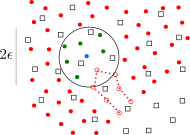
\includegraphics[width=0.5\textwidth]{Figure-Particle-failed}
  \caption{Scheme of a linear cohesive law, where the shaded area is
    $G_f$, $f_t$ is the tensile strength, and $w_c$ is the critical
    opening displacement.}
  \label{fig:Failed-particles}
\end{figure}
%%%%%%%%%%%
Other parameters are, the mass of the neighborhood $m_p^{k+1}$, the
current free-energy density per unit mass  $W_q^{k+1}$ and finally a
normalizing constant $C_{\epsilon}$. 
The failure criterion consist in to consider the material point fails
when $G_p^{k+1}$ surpasses a critical energy release rate that
measures the material-specific energy, $G_F$. The convergence of this
approach has been analyzed by Schmidt {\it et al.}
(2009)\cite{Schmidt_2009}, who proofed that it converges to the Griffith
fracture when discretization size tends to zero. It is necessary to
point out that when a material point overpass the critical energy, its
contribution to the internal forces vector is set to zero, but its
contribution to the mass matrix is preserved.\\

As can be noticed, the eigenerosion algorithm relies over an energetic
failure criterion. Because of this, unrealistic stress
concentration (higher than tensile strength) appears in quasi-brittle
materials \cite{Navas_2017_ES}. To overcome this limitation, the
aforementioned authors proposed the concept of eigensoftening to take
in to account the gradual failure in quasi-brittle materials. The idea
behind this concept is inspired in the cohesive fracture. This gradual
failure criterion is plotted in figure \label{fig:Damage-ft-wc}, where
a linear decreasing cohesive law is presented to illustrate the
concept earlier described. In the picture, the shaded region represents
the static fracture energy per unit of area, $G_F$. Notice how a
cohesive crack appears when the maximum tensile strength, $f_t$ is
reached. Once the opening displacement $w$ reach the value of the
critical crack displacement $w_c$, a stress-free crack is
attained. For intermediate values, $w_n$, a damage value between zero
and one represents the extension to which the material has failed.
%%%%%%%%%%%
\begin{figure}
  \centering
  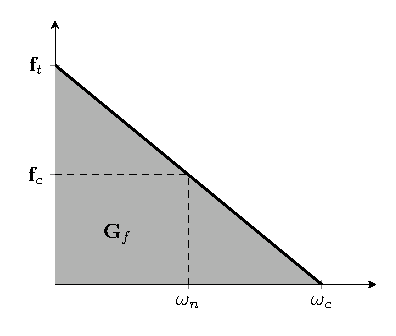
\includegraphics[width=0.5\textwidth]{Figure-Damage}
  \caption{Scheme of a linear cohesive law, where the shaded area is
    $G_f$, $f_t$ is the tensile strength, and $w_c$ is the critical
    opening displacement.}
  \label{fig:Damage-ft-wc}
\end{figure}
%%%%%%%%%%%
For the eigensoftening algorithm, a strength criterion for crack
initialization was adopted. Particularly the maximum principal stress
theory for brittle fracture was considered by authors
\cite{Navas_2017_ES}. With that purpose, the variation of the averaged
strain energy density in the $\epsilon$-neighborhood of the material point
$\vec{x}_p^{k+1}$ can be obtained as
\begin{equation}
  \label{eq:variation-averaged-strain-energy-density}
  \delta W_{\epsilon,p} = \frac{\partial G_p}{C_{\epsilon}} =
  \frac{1}{m_p} \sum_{x_q^{k+1} \in
  B_{\epsilon}(x_p^{k+1})} m_q \tens{\sigma}_{q,I} \delta \tens{\epsilon}_q,
\end{equation}
where $\tens{\sigma}_{q,I}$ is the maximum principal stress of each
material point in the $\epsilon$-neighborhood. In this point in
introduced an effective strain $\varepsilon_q$, such the variation of
the local strain energy can be obtained as $\delta W_q = \sigma_{q,1}
\delta\varepsilon_q$. Now with the assumption that the effective
strain of each material point at every time step is constant in the
neighborhood of $\vec{x}_p^{k+1}$, the equation 
\eqref{eq:variation-averaged-strain-energy-density} can be simplified
 to
\begin{equation}
  \label{eq:variation-averaged-strain-energy-density-simpli}
  \delta W_{\epsilon,p} =
  \frac{\delta \tens{\epsilon}_p}{m_p} \sum_{x_q^{k+1} \in
  B_{\epsilon}(x_p^{k+1})} m_q \tens{\sigma}_{q,I}. 
\end{equation}
Consequently it is possible to define an equivalent critical stress at the
material point $\vec{x}_p^{k+1}$as
\begin{equation}
  \label{eq:equivalent-critical-stress}
  \tens{\sigma}_{\epsilon,p} =
  \frac{1}{m_p} \sum_{x_q^{k+1} \in
  B_{\epsilon}(x_p^{k+1})} m_q \tens{\sigma}_{q,I}, 
\end{equation}
where $m_p$ is the total mass of the $\epsilon$-neighborhood
\begin{equation}
  \label{eq:averaged-mass}
  m_p = \sum_{x_q^{k+1} \in B_{\epsilon}(x_p^{k+1})} m_q.
\end{equation}
This definition of the equivalent critical stress leads to a
definition of the averaged strain energy in terms of the averaged
strain as $\delta W_{\epsilon,p} =
 \tens{\sigma}_{\epsilon,p}\ \delta\varepsilon_p$. The softening behaviour is
activated once $\tens{\sigma}_{\epsilon,p}^{k+1}$ surpasses the
tensile strength, $f_t$. This consists in a reduction of the internal
forces as,
 \begin{equation}
   \label{eq:f-int-damaged}
   f^{int}_I = \sum_p (1 - \chi_p)\ \tens{\sigma}_{p}^{k+1} \cdot
   \Grad{N_{Ip}}\ \Omega_p
 \end{equation}
where $\chi_p$ and $\Omega_p$ are respectively the damage or softening
variable and the volume for each material point $p$. $\chi_p$ takes
values between zero (an intact material) and one (completely failed
material points). For the case of a linear softening such the sketched in the Figure \ref{fig:Damage-ft-wc}, $\chi_p$ is computed as,
 \begin{equation}
   \label{eq:damaged-variable-chi}
   1 - \chi = \frac{f_n}{f_t} = 1 - \frac{w_n}{w_c}\ \rightarrow\ \chi
   = \frac{w_n}{w_c}.
 \end{equation}
In analogy to the band crack model presented by
Bazant~\cite{Bazant83}, Navas {\it et al.} \cite{Navas_2018_ES}
\cite{Navas_2017_ES} introduced a band width parameter $h_{\epsilon}$.
Concerning this parameter, a typical value of it is between two and
four times the maximum size of the aggregates, in the case of
concrete as brittle material. The effective fracture strain
$\varepsilon_{\epsilon,f}$ is defined as the difference between the strain at crack initialization,
$\varepsilon_1(\vec{x}_p^{0})$, and the current strain, $\varepsilon_1(\vec{x}_p^{k+1})$, for material point $p$. Also,
$\varepsilon_{\epsilon,f}$ can be represented as the current crack
opening $w_n$ within the band width, $h_{\epsilon}$. Therefore, 
\begin{equation}
  \label{eq:effective-fracture-strain}
  \varepsilon_{\epsilon,f} = \varepsilon_1(\vec{x}_p^{k+1}) -
  \varepsilon_1(\vec{x}_p^{0}) = \frac{w_n}{h_{\epsilon}}
\end{equation}
Introducing \eqref{eq:effective-fracture-strain} in
\eqref{eq:damaged-variable-chi}, the damage variable can be computed
as,
\begin{equation}
  \label{eq:damage-variable-chi-II}
\chi = \frac{\varepsilon_{\epsilon,f}\ h^{\epsilon}}{w_c}.  
\end{equation}
The function of $\chi$ presented in \eqref{eq:damage-variable-chi-III}
represents a linear softening behaviour. For a general case, the
damage variable can be expressed in terms of the following variables,
\begin{equation}
  \label{eq:damage-variable-chi-III}
  \chi = \chi(\varepsilon_{\epsilon,f}, h^{\epsilon}, f_t, w_c, G_f)
\end{equation}
Implementation details can be consulted in \ref{sec:eigens-algor-1}
%%%%%%%%%%%%%%%%%%%%%%%%%%%%%%%%%%%%%%%%%%%%%%%%%%%%%%%%%%%%%%%%%%%%%%%%%
\section{Cases of study and discussion}
\label{sec:3}

As noticed in \cite{Zhang_EE_2020}, the EigenMPM have two important
shortcomings. The first is the presence of stress instabilities even
with \acrshort{gimp} shape functions. To overcome it, \acrshort{lme}
approximants are introduced as an
alternative to the existing interpolation techniques. Its
impressive performance mitigating spurious stress oscillations
\cite{Wobbes2020} under the \acrshort{mpm} framework help to enhance
notoriously the quality of the results as we can see in Section
\ref{sec:3.1}. Where both interpolation techniques
are compared by carry out an eigenerosion simulation. The second
limitation is concerning its inability to simulate properly quasi-brittle
fracture \cite{Navas_2018_ES}. It can be solved thorough the
eigensoftening algorithm described in Section \ref{sec:2.3}. A proof
of it is exposed in Section \ref{sec:3.3}, where experimental results
of a drop-weight impact test are compared with those produced by
eigensoftening computations.

\subsection{Edge-cracked square panel in mode I}
\label{sec:3.1}

This problem here presented is devoted to compare how much \acrshort{lme}
approximants are able to improve the result \textit{versus} standard
linear interpolation. It consists in a square plate of size $H = 1$ containing
an initial edge crack of length $0.25 \cdot H$ loaded in a pure mode I
by displacement control on the outer flanks of the plate, Figure
\ref{fig:geometry-cracked-panel-mode-I}.
%%%%%%%%%%%%%%%%%%%%%%%%%%%%%%%%%%%%%%%%%%%%%%%%%%
\begin{figure}
  \centering
  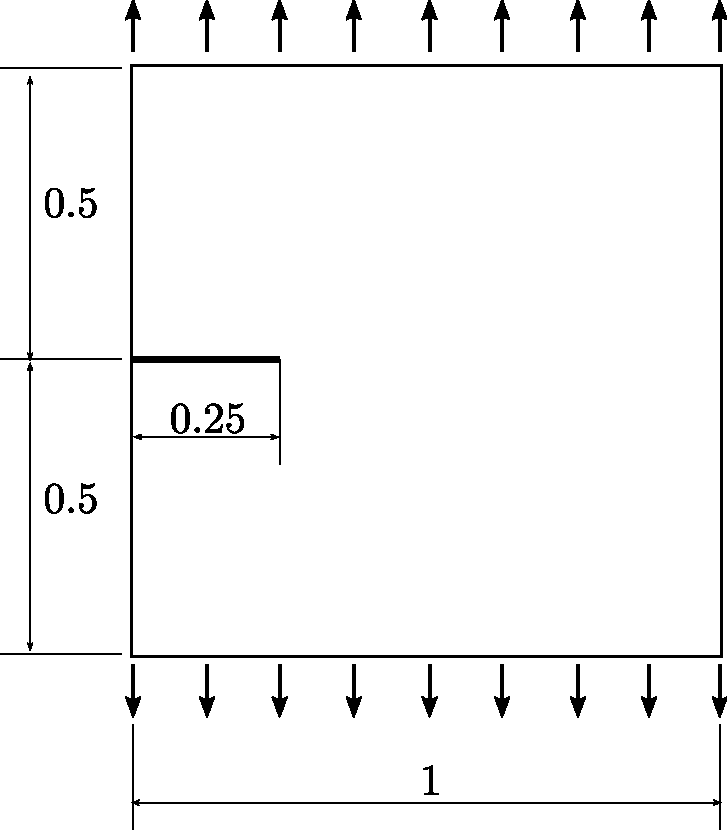
\includegraphics[width=0.4\textwidth]{Figure-Mode_I}
  \caption{Geometry and boundary condition of the drop-weight impact test.}
  \label{fig:geometry-cracked-panel-mode-I}
\end{figure}
%%%%%%%%%%%%%%%%%%%%%%%%%%%%%%%%%%%%%%%%%%%%%%%%%%
The constitutive model consider for numerical experiment is a
linear-elastic Hookean material, where Young's modulus \gls{E} = 1.06, the
Poisson's ratio \gls{nu} = 0.333, and critical energy-release rate
\gls{Gf} = 0.0001. This set of parameters was taken from \cite{Pandolfi_2012}. In
\acrshort{mpm}, two different discretization are required. In one hand
a cartesian grid of nodes is consider with a nodal spacing value of
0.025. On the other hand, the plate will be modeled with a initial
layout of four particles per element and occupying the Gauss quadrature
positions.\\

Figure \ref{fig:Reactions-cracked-panel-mode-I} clearly shows the
presence of wiggles in both loading and fracture stages
in the reaction-displacements curve when linear interpolation
technique is used. In contrast, \acrshort{lme} simulation does not
exhibit these spurious oscillations and remains linear. Besides that,
linear interpolation produces stiffer results than
\acrshort{lme}. This can be attributed to imprecision in the stress
field due to grid-crossing phenomena.\\
%%%%%%%%%%%%%%%%%%%%%%%%%%%%%%%%%%%%%%%%%%%%%%%%%%%%%%
\begin{figure}
  \centering
  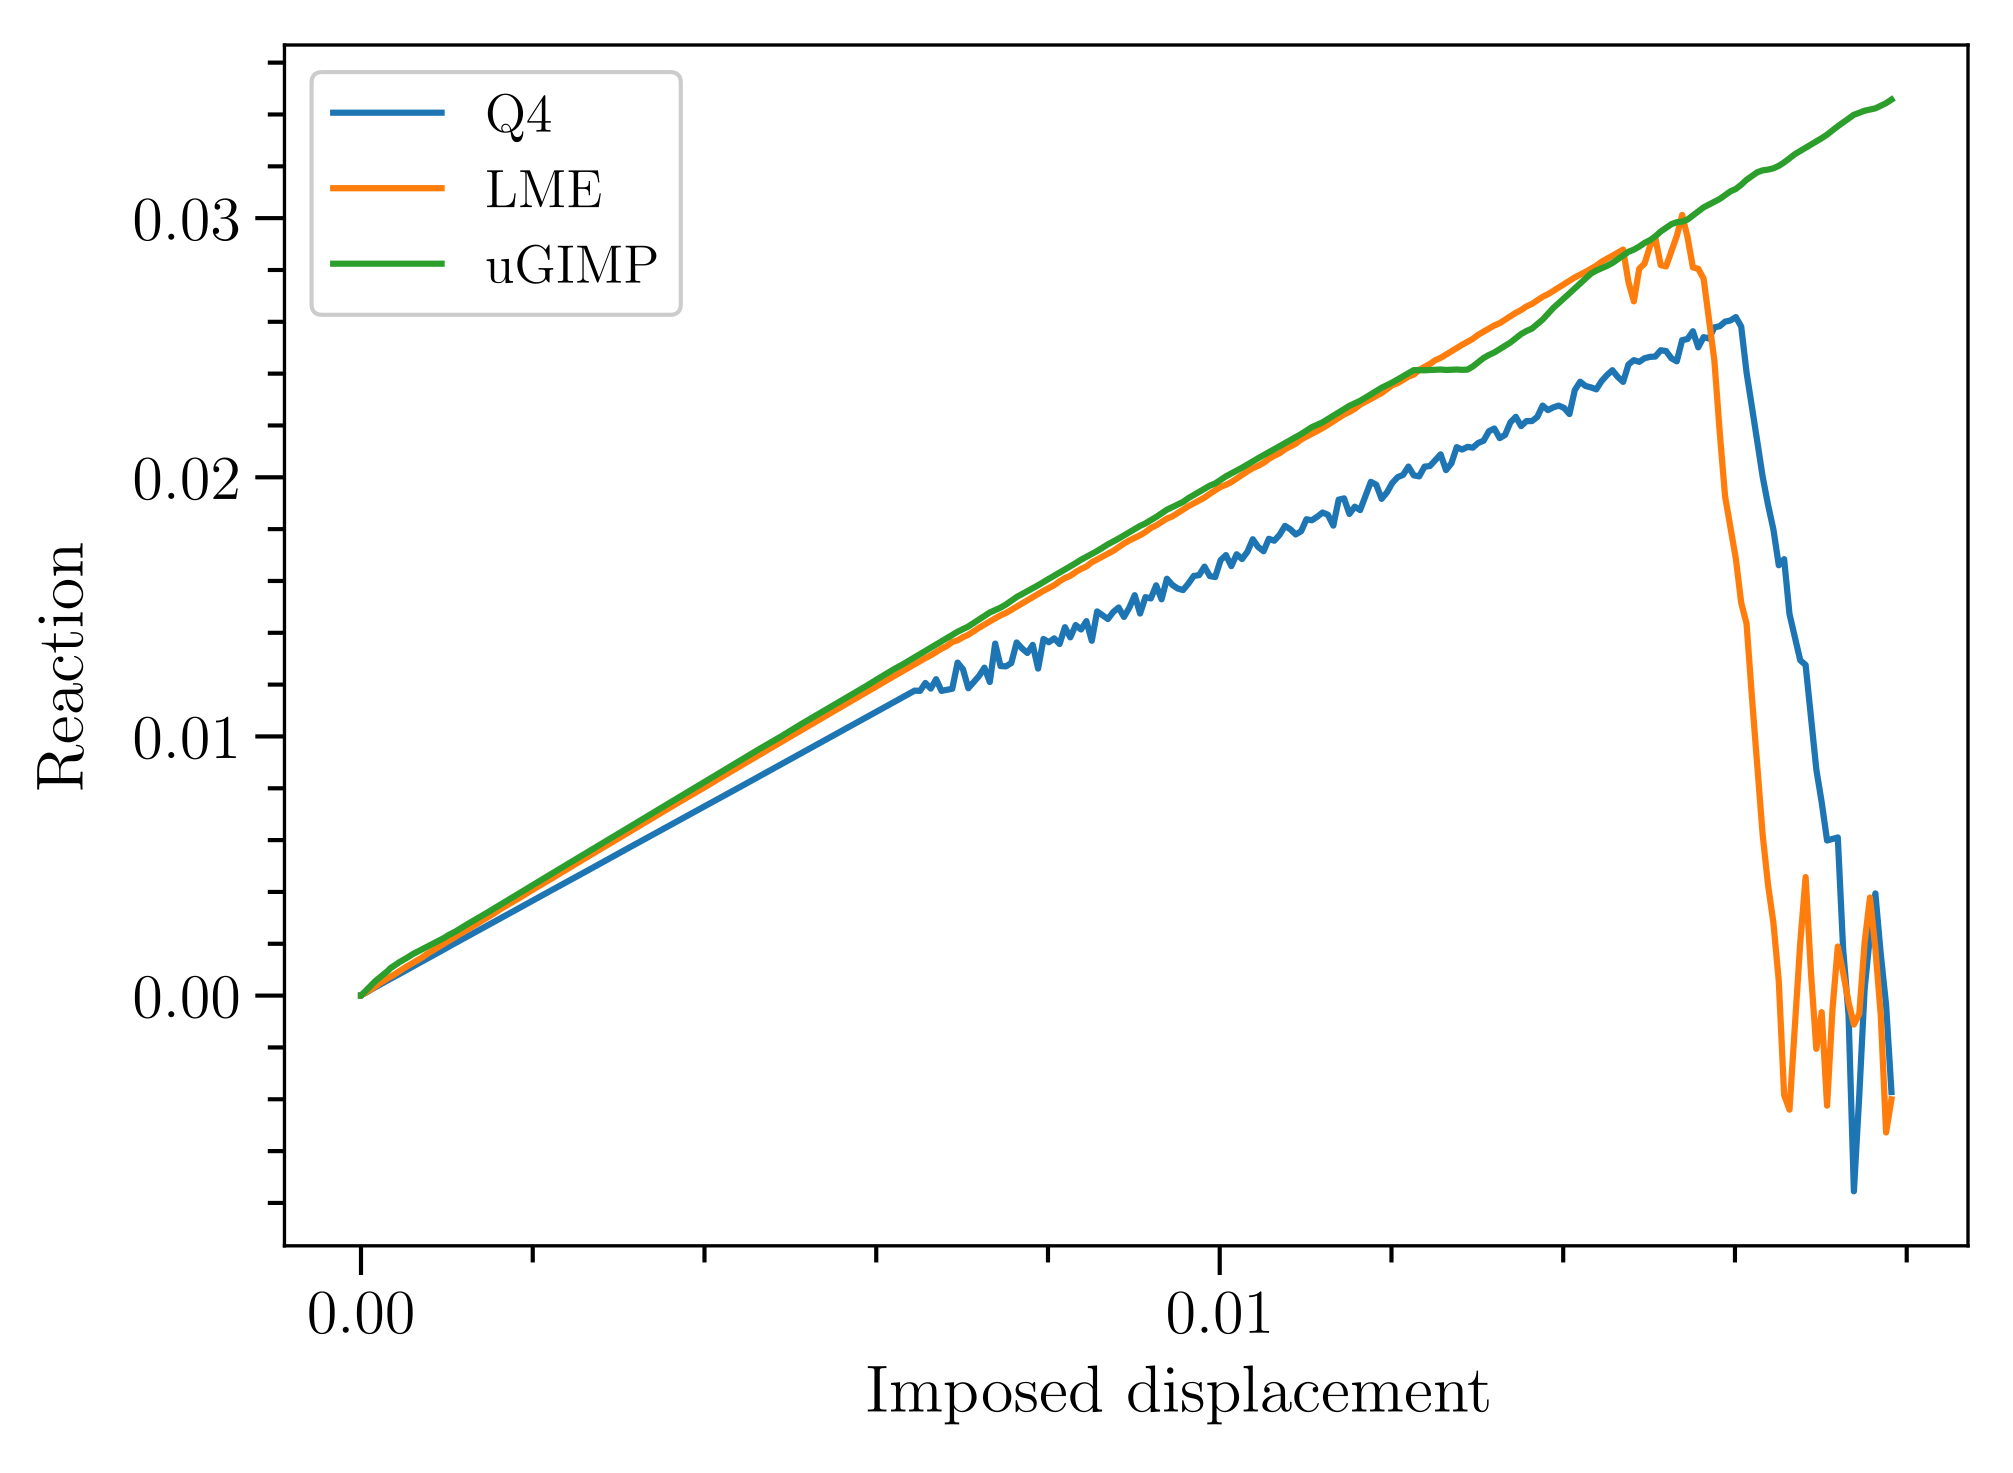
\includegraphics[width=0.8\textwidth]{Figure-Reactions-Mode-I}
  \caption{Evolution of the reaction forces plotted \textit{versus}
    the imposed displacement for linear interpolation technique and
    the \acrshort{lme} approximants.}
  \label{fig:Reactions-cracked-panel-mode-I}
\end{figure}
%%%%%%%%%%%%%%%%%%%%%%%%%%%%%%%%%%%%%%%%%%%%%%%%%%%%%%
On the other hand, Figure \ref{fig:Stress-cracked-panel-mode-I}
exhibits more clearly the difference between linear interpolation and
\acrshort{lme}, since numerical instability becomes rather significant
when particles crosses the boundary of the element in the linear
case. Although this behavior does not affect significantly to the peak
stress value in a hookean material \cite{Zhang_EE_2020}, if
hyperelastic materials are consider for future simulations,
inaccuracies in the stress field could affect dramatically to the
final result. On the other hand \acrshort{lme} produces soft stress
field evolution even after breaking.
%%%%%%%%%%%%%%%%%%%%%%%%%%%%%%%%%%%%%%%%%%%%%%%%%%%%%%
\begin{figure}
\centering
\subfigure[t = 25]{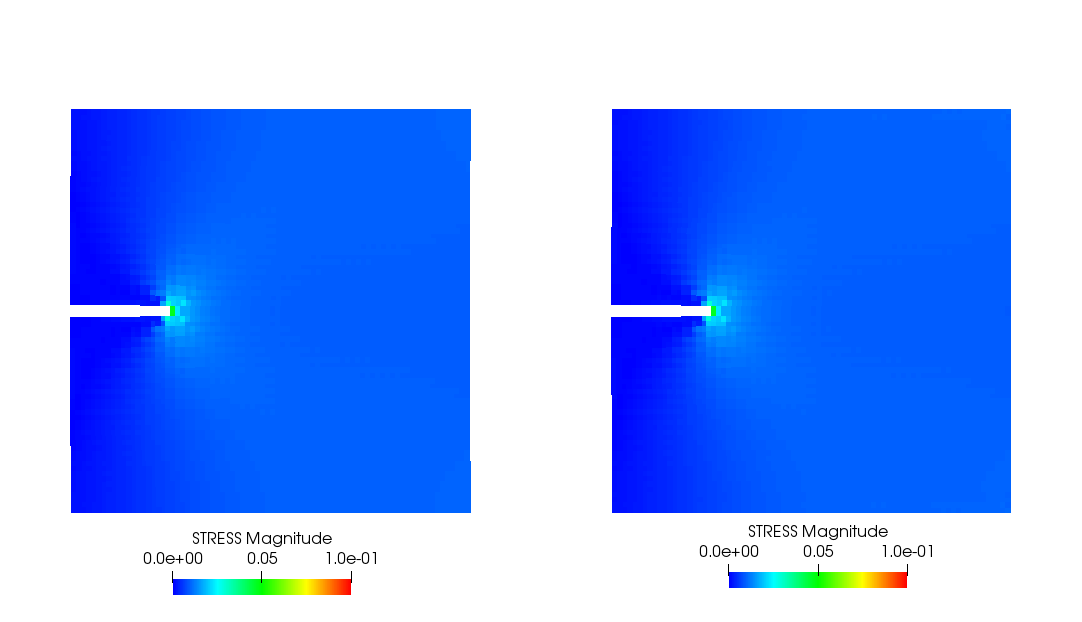
\includegraphics[width=0.73\textwidth]{./Figure-Stress-0100-mode-I.png}}
\subfigure[t = 60]{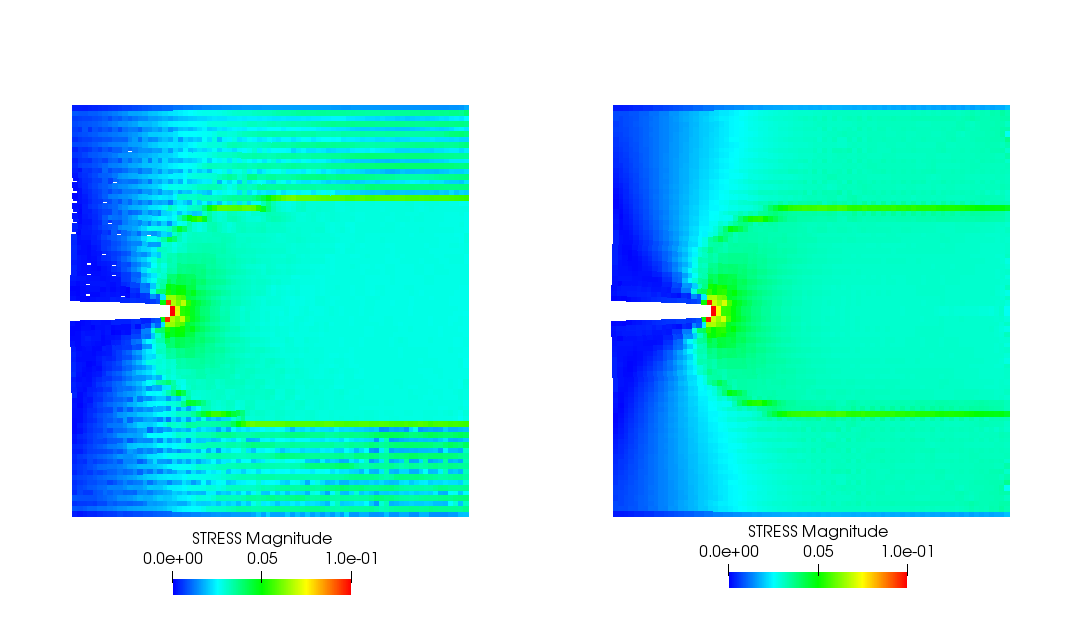
\includegraphics[width=0.73\textwidth]{./Figure-Stress-0250-mode-I.png}}
\subfigure[t = 100]{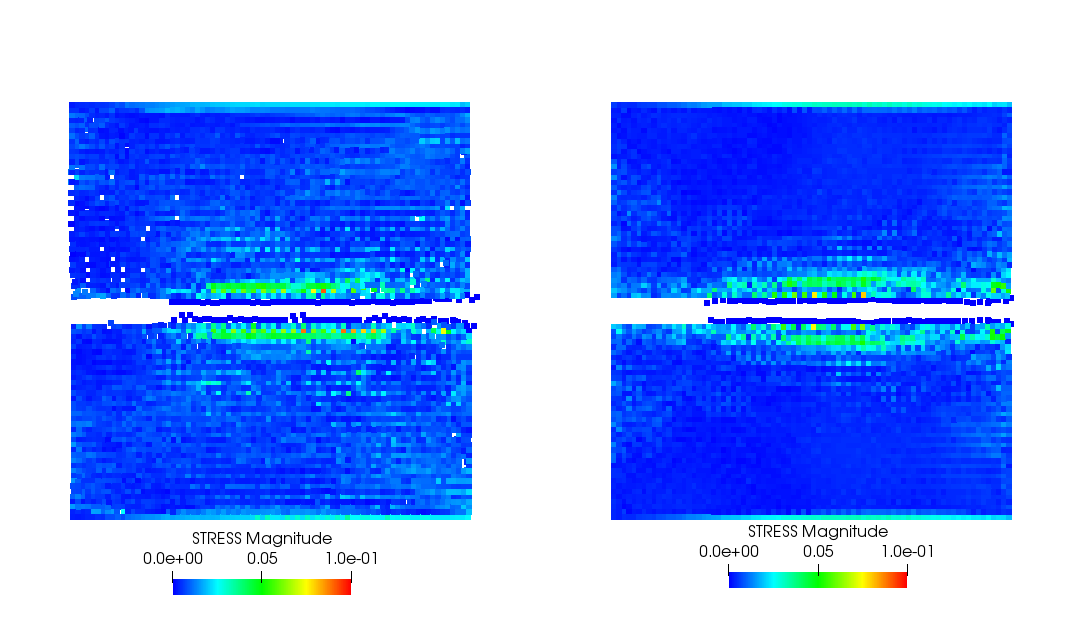
\includegraphics[width=0.73\textwidth]{./Figure-Stress-0398-mode-I.png}}
\caption{Evolution of the stress tensor magnitude for linear
  interpolation (pictures in the left side), and \acrshort{lme}
  (pictures in the right side). Both simulations performed with an
  eigenerosion algorithm.}
\label{fig:Stress-cracked-panel-mode-I}
\end{figure}
%%%%%%%%%%%%%%%%%%%%%%%%%%%%%%%%%%%%%%%%%%%%%%%%%%%%%%
An important consideration regarding the presence of oscillations once
both parts of the panel are separated, Figure
\ref{fig:Reactions-cracked-panel-mode-I}. These phenomena should not be
attributed to the eigenerosion algorithm since the fracture process is
over. They are due to the dynamic nature of the solver.  

\subsection{Drop-weight impact test}
\label{sec:3.2}

Once the accuracy of the \acrshort{lme} approximants have been proven
in Section \ref{sec:3.1}, henceforth will be adopted without comparing
with linear interpolation. Therefore this section is devoted to proof
the accuracy of the eigensoftening algorithm to simulate the behavior
of quasi-brittle materials under dynamic loading. An example of this
load case is the three-point bending test on a notched beam is
conducted under impact loading. This kinds of experiments are
challenging to reproduce numerically with an explicit solver since
fracture occurs in a period of milliseconds and high strength
materials are involved. Accordingly, really small time steps are
required to achieve a simulation numerically stable. Additionally,
this kind of simulations traditionally require the implementation of
contact algorithm to reproduce the hammer impact in the beam. In the
\acrshort{mpm}, the implementation of this feature can be bypassed to
obtain preliminary results. Nevertheless, this kind of algorithm could
be implemented to get ever more accurate solutions. Although this is
out of the scope of this document, future research of authors will overcome this
limitation.\\

As in the study of Zhang {\it et al.} \cite{Zhang_2009,Zhang_2010a},
an impact hammer of 120.6 kg was employed to drop it at an impact
speed of 881 mm/s. The beam dimensions where 100 mm x 100 mm (B x D)
in cross section, and 420 mm in total lenght (L). The initial
notch-depth ratio was approximately 0.5, and the span, S, was fixed at
300 mm during the tests, see Figure
\ref{fig:geometry-drop-weight-impact-test}.
%%%%%%%%%%%%%%%%%%%%%%%%%%%%%%%%%%%%%%%%%%%%%%%%%%
\begin{figure}
  \centering
  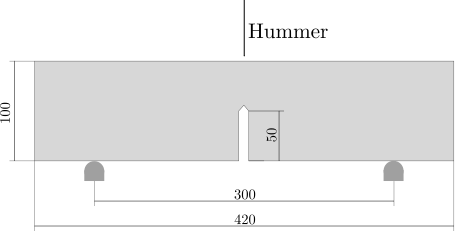
\includegraphics[width=0.8\textwidth]{./Figure-impact-test}
  \caption{Geometry and boundary condition of the drop-weight impact test.}
  \label{fig:geometry-drop-weight-impact-test}
\end{figure}
%%%%%%%%%%%%%%%%%%%%%%%%%%%%%%%%%%%%%%%%%%%%%%%%%%
The material adopted for the simulation was characterised by Navas
{\it et al.}~\cite{Navas_2017_ES}, and the material properties, such
as the material density, \gls{rho}, the compressive strenght, \gls{fc},
the tensile strenght \gls{ft}, the specific fracture energy, \gls{Gf},
and the elastic modulus \gls{E} are given in table \ref{tab:concrete-properties}.\\
%%%%%%%%%%%%%%%%%%%%%%%%%%%%%%%%%%%%%%%%%%%%%%%%% 

\begin{table}
  \centering
  \begin{tabular}[]{c c c c c c c}
    \hline
      &   $\rho$   & $\text{f}_c$ & $\text{f}_t$ & $G_F$ &   E   & $\text{d}_{max}$ \\
      & (kg/m$^3$) &     (MPa)    &     (MPa)    & (N/m) & (GPa) & (mm) \\
    \hline
Value &    2368    &     102.7    &      5.4     &  141  &   31  &  12 \\
    \hline
  \end{tabular}
  \caption[Mechanical properties of thje concrete]{Mechanical
    properties of the high strenght concrete.}
  \label{tab:concrete-properties}
\end{table}
%%%%%%%%%%%%%%%%%%%%%%%%%%%%%%%%%%%%%%%%%%%%%%%%%
For the present research, a 2D setting of the experiment has been
adopted. Both the hammer and the concrete beam are explicitly
represented. Several levels of discretization were required to assess
the objectiveness of the obtained results. The results here exposed
are from a discretization of 30616 material points and 6297 nodes. To
achieve better results, an unestructured grid layout has been adopted
focusing the minimum nodal spacing, 0.47 mm, in the middle of the beam and in
the impact surface of the hammer. For this simulation, $\gamma$ was
fixed to 6.\\

First the reaction and impact forces are validated against their
experimental counterparts. Since the impact forces applied by the
hammer and the reaction forces at the two supports were experimentally
measured, they are compared with numerical ones in Figure
\ref{fig:Reactions-Forces-impact-test}. 
%%%%%%%%%%%%%%%%%%%%%%%%%%%%%%%%%%%%%%%%%%%%%%%%%%%%%% 
\begin{figure}
  \centering
  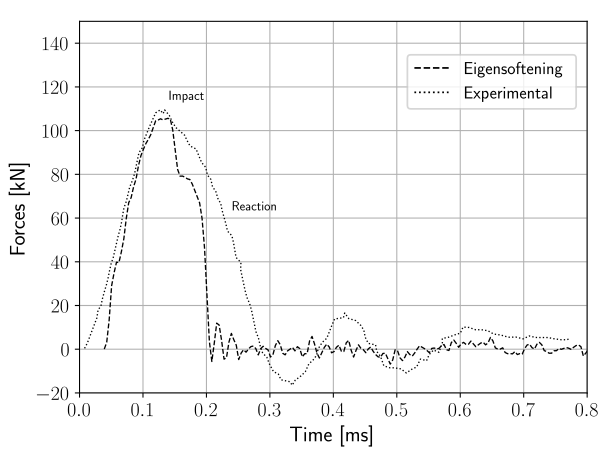
\includegraphics[width=0.8\textwidth]{Figure-impact-test-Forces-Time}
  \caption{Evolution of the reaction forces plotted \textit{versus}
    the imposed displacement for linear interpolation technique and
    the \acrshort{lme} approximants.}
  \label{fig:Reactions-Forces-impact-test}
\end{figure}
%%%%%%%%%%%%%%%%%%%%%%%%%%%%%%%%%%%%%%%%%%%%%%%%%%%%%%
Note that the general trend of both forces are correctly
captured. Observe that in experimental solution the delay between
impact peak and reactions peak does not agree with the numerical
ones. On the other hand, if the delay is computed analytically through
concrete wave speed is much closer to the numerical results. A
feasible explanation to this unexpected result can due the composite
nature of the concrete. Another discrepancy is in the much higher
values of maximum impact and reaction forces in numerical than in
experimental. In this case, this is a consequence of over-rigidity
in the supports. Therefore, this results can be improved in future research
by a suitable contact algorithm.\\

And finally horizontal stress distributions and crack propagation are
extracted, see Figure \ref{fig:Stress-vs-damage-impact-test}. Stress
evolution agrees with the results obtained by \cite{Navas_2017_ES}
under the \acrshort{otm} framework. Two additional considerations about
this results are concerning the interpolation technique. In one hand,
in the opposite to the \acrshort{ugimp} shape function, \acrshort{lme}
allows unstructured grids. This is a remarkable benefit for this kind
of simulations since the majority of the computational effort is
clearly localised in a tiny region of the domain. And in the other
hand there is the possibility to reduce the shape function support to avoid
a material point in one side of the crack is affected by those in the
other side of the crack. 
%%%%%%%%%%%%%%%%%%%%%%%%%%%%%%%%%%%%%%%%%%%%%%%%%%%%%%
\begin{figure}
\centering
\subfigure[t = 0.27 ms]{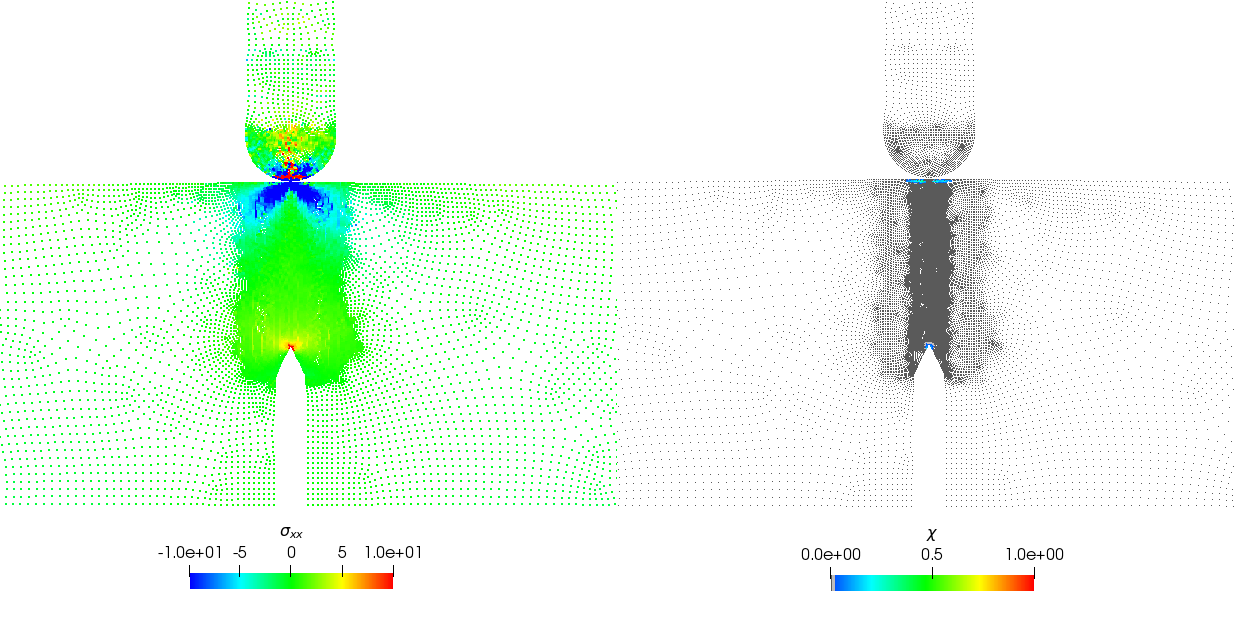
\includegraphics[width=0.83\textwidth]{./Figure-impact-test-Damage-vs-Stress-0060}}
\subfigure[t = 0.36 ms]{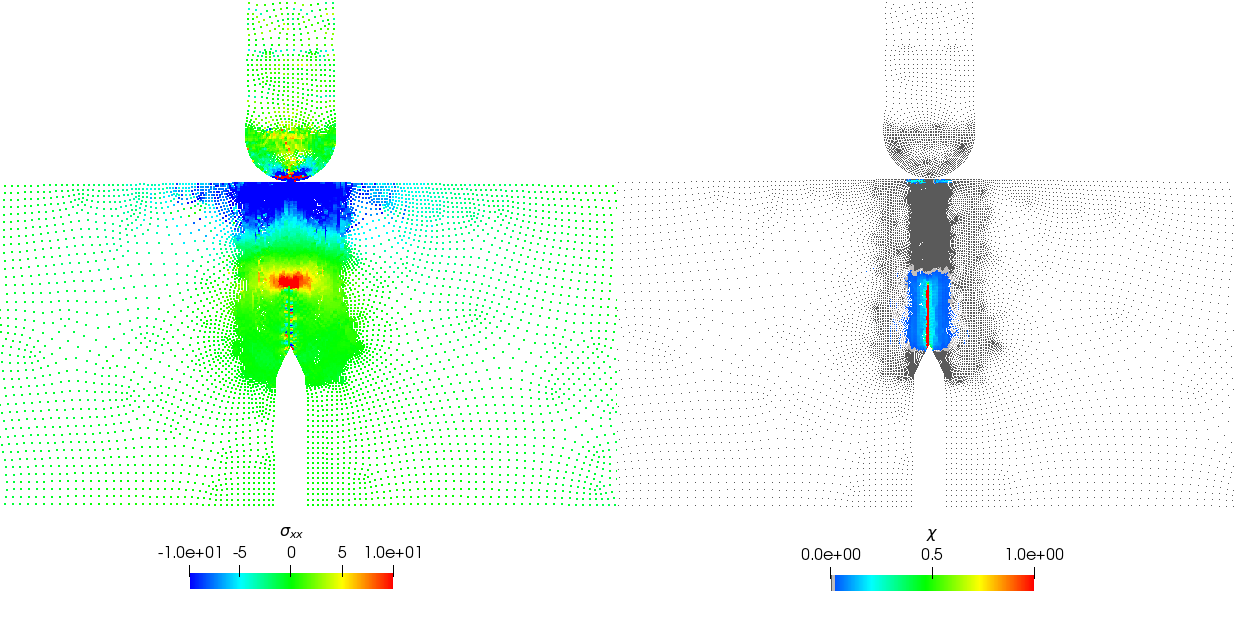
\includegraphics[width=0.83\textwidth]{./Figure-impact-test-Damage-vs-Stress-0080}}
\subfigure[t = 0.45 ms]{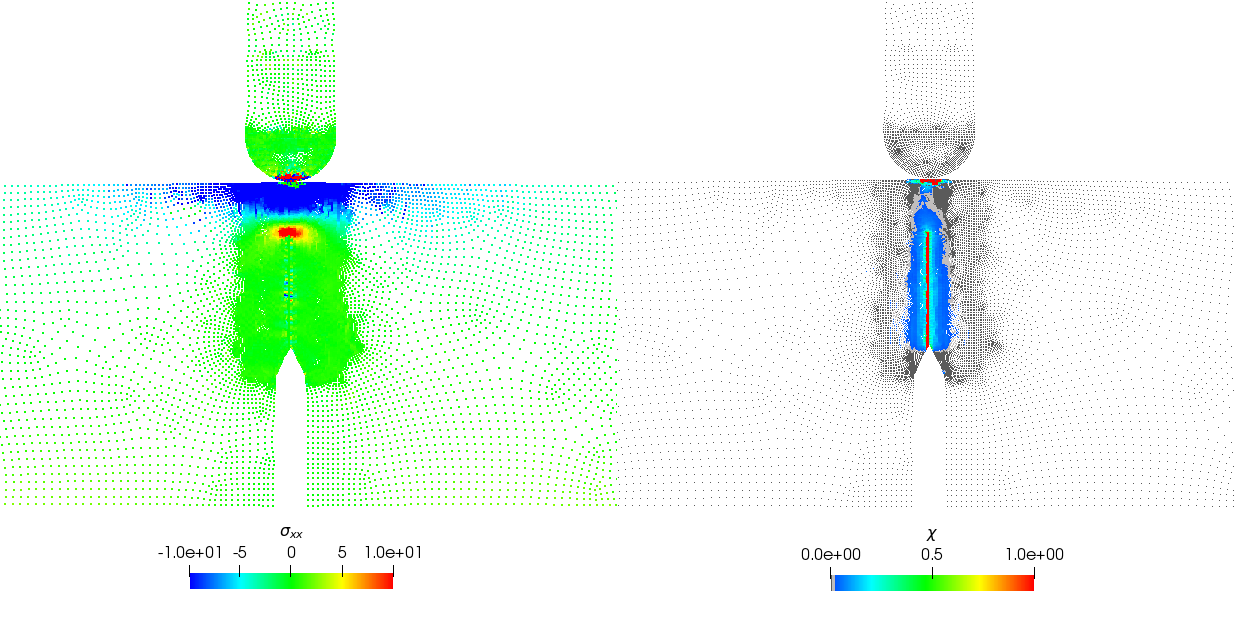
\includegraphics[width=0.83\textwidth]{./Figure-impact-test-Damage-vs-Stress-0100}}
\caption{Evolution of the stress tensor magnitude for linear
  interpolation (pictures in the left side), and \acrshort{lme}
  (pictures in the right side). Both simulations performed with an
  eigenerosion algorithm.}
\label{fig:Stress-vs-damage-impact-test}
\end{figure}
%%%%%%%%%%%%%%%%%%%%%%%%%%%%%%%%%%%%%%%%%%%%%%%%%%%%%%

\section{Conclusions}
\label{sec:4}
Based on the EigenMPM approach to fracture proposed by Zhang {\it et al.}
\cite{Zhang_EE_2020}, we have proposed two addition improvements which
solves the shortcomings presented in the original concept. First by
bring to the \acrshort{mpm} framework the concept of eigensoftening,
which allow to consider gradual failure process of each material
point. This concept can be compared with a cohesive law in the context
of cohesive fracture. Furthermore, more elaborated damage curves can
be designed to describe the failure process in more sophisticated
materials. In this direction, an interesting future improvement of the
algorithm would be the ability to simulate of crack patterns in
composite material such carbon fiber. This leads a challenging
research topic. Secondly, \acrshort{lme} is employed to remove from
the solution those wiggles due to inaccuracies in the stress
integration. This interpolation technique could help to improve
results in fracture propagation by adapting it thorough the
deformation gradient. \textit{A priori} this will enhance the already
impressive localisation properties of eigensoftening and eigenerosion
algorithms. 

\section*{Acknowledgements}
The financial support to develop this research from the Ministerio de
Ciencia e Innovaci\'on, under Grant No. BIA-2016-76253 is greatly
appreciated. The first and the second authors also acknowledge the
fellowship Fundaci\'on Agust\'in de Betancourt and Juan de la Cierva
(FJCI-2017–31544) respectively.

\appendix
%\addappheadtotoc
%\appendixpage
%\renewcommand{\theequation}{\Alph{section}.\arabic{equation}}

\section{Explicit Newmark Predictor-Corrector algorithm}
\label{sec:expl-pred-corr}
\begin{algorithm}[H]
  \DontPrintSemicolon
    %%%%%%%%%%%%%%%%%%%%%%%%%%%%%%%%%%%%%%%%%%%%%%%%%%%%%%%%%%%%%%%%%%%%%%%%%%%%%%%%%%%%%%
    \textbf{Update mass matrix :} $ \tens{m}_{I} = N_{Ip}^{k}\ m_p$ \;
    %%%%%%%%%%%%%%%%%%%%%%%%%%%%%%%%%%%%%%%%%%%%%%%%%%%%%%%%%%%%%%%%%%%%%%%%%%%%%%%%%%%%%% 
    \textbf{Explicit Newmark Predictor :}
    \begin{equation*}
      \vec{v}_I^{pred} = \frac{ N_{Ip}^{k} m_p (\vec{v}_p^k + (1 - \gamma)\ \Delta t\ \vec{a}_p^k)}{m_I}
    \end{equation*}\;
    %%%%%%%%%%%%%%%%%%%%%%%%%%%%%%%%%%%%%%%%%%%%%%%%%%%%%%%%%%%%%%%%%%%%%%%%%%%%%%%%%%%%%% 
    \textbf{Impose essential boundary conditions :} At the fixed
    boundary, set $\vec{v}_{I}^{pred} = 0$.\; 
    %%%%%%%%%%%%%%%%%%%%%%%%%%%%%%%%%%%%%%%%%%%%%%%%%%%%%%%%%%%%%%%%%%%%%%%%%%%%%%%%%%%%%% 
    \textbf{Deformation tensor increment calculation :}
    \begin{equation*}
      \Delta \tens{\varepsilon}_{p}^{k+1} = \Delta t\
        \dot{\tens{\varepsilon}_{p}}^{k+1} = \Delta t\ \left[ \vec{v}_{I}^{pred} \otimes
        \Grad{N_{Ip}^{k+1}} \right]^s
    \end{equation*} \;
    %%%%%%%%%%%%%%%%%%%%%%%%%%%%%%%%%%%%%%%%%%%%%%%%%%%%%%%%%%%%%%%%%%%%%%%%%%%%%%%%%%%%%% 
    \textbf{Update the density field :} $\rho_p^{k+1} =
    \frac{\rho_p^k}{1 + \mathit{tra}\left[\Delta\tens{\varepsilon}_{p}^{k+1}\right]}.$\;
    %%%%%%%%%%%%%%%%%%%%%%%%%%%%%%%%%%%%%%%%%%%%%%%%%%%%%%%%%%%%%%%%%%%%%%%%%%%%%%%%%%%%%% 
    \textbf{Compute stress field and update damage parameter}\;
    %%%%%%%%%%%%%%%%%%%%%%%%%%%%%%%%%%%%%%%%%%%%%%%%%%%%%%%%%%%%%%%%%%%%%%%%%%%%%%%%%%%%%% 
    \textbf{Balance of forces calculation :} Calculate the total grid
    nodal force $\vec{f}_{I}^{k+1} = \vec{f}_{I}^{int,k+1} + \vec{f}_{I}^{ext,k+1}$.\;
    %%%%%%%%%%%%%%%%%%%%%%%%%%%%%%%%%%%%%%%%%%%%%%%%%%%%%%%%%%%%%%%%%%%%%%%%%%%%%%%%%%%%%% 
    \textbf{Explicit Newmark Corrector :}
    \begin{equation*}
      \vec{v}_{I}^{k+1} = \vec{v}_{I}^{pred} + \gamma\ \Delta t\ \frac{\vec{f}_{I}^{k+1}}{\tens{m}_I^{k+1}}  
    \end{equation*}\;
    %%%%%%%%%%%%%%%%%%%%%%%%%%%%%%%%%%%%%%%%%%%%%%%%%%%%%%%%%%%%%%%%%%%%%%%%%%%%%%%%%%%%%%
    \textbf{Update particles lagrangian quantities :}
    \begin{align*}
      &\vec{a}_p^{k+1} = \frac{N_{Ip}^k\vec{f}_{I}^{k}}{\tens{m}_I^k}\\
      &\vec{v}_p^{k+1} = \vec{v}_p^n + \Delta t\
        \frac{N_{Ip}^k\
        \vec{f}_{I}^{k}}{\tens{m}_I^k}\\
      &\vec{x}_p^{k+1} = \vec{x}_p^n + \Delta t\
         N_{Ip}^k\ \vec{v}_{I}^{k} +
        \frac{1}{2}\Delta t^2\ \frac{N_{Ip}^k\
        \vec{f}_{I}^{k}}{\tens{m}_I^k}
    \end{align*}\;
    %%%%%%%%%%%%%%%%%%%%%%%%%%%%%%%%%%%%%%%%%%%%%%%%%%%%%%%%%%%%%%%%%%%%%%%%%%%%%%%%%%%%%% 
    \textbf{Reset nodal values}\;
    %%%%%%%%%%%%%%%%%%%%%%%%%%%%%%%%%%%%%%%%%%%%%%%%%%%%%%%%%%%%%%%%%%%%%%%%%%%%%%%%%%%%%% 
    \label{alg-epc}
    \caption{Explicit Newmark Predictor-Corrector scheme}
\end{algorithm} 


\section{Eigensoftening Algorithm}
\label{sec:eigens-algor-1}

\begin{algorithm}[H]
  \DontPrintSemicolon
  \KwInput{For each $p$, $\epsilon$-neighbourhood, $f_{t,p}$, $h_{\epsilon,p}$, $w_c$}
  \KwOutput{Return damage parameter $\chi := \{\chi_p\}$}
  % \KwData{Testing set $x$}
  $\chi_p \leftarrow \chi_p^{k}$ \;
  \For{$p$ to $N_p$}
  {
    \If{$\chi_p = 0$ \AND $\epsilon_{f,p} = 0$}
    {
      \For{$q \in B_{\epsilon,p}$}
      {
        $\sigma_{q,I} \leftarrow \text{getEigenvaluesOf}(\sigma_{q})$ \;
        \If{$\chi_q < 1$}
        {
          $\sum m_p\sigma_{p,I} \leftarrow \sum m_p\sigma_{p,I} + m_q\sigma_{q,I}$ \;
        }
        $m_p \leftarrow m_p + m_q$ \;
      }
      $\sigma_{p,\epsilon} \leftarrow \frac{1}{m_p} \sum m_p\sigma_{p,I}$\;
      \If{$\sigma_{p,\epsilon} > f_{t,p}$}
      {
        $\epsilon_{f,p} = \epsilon_{I,p}$ \;  
      }
      \ElseIf{$\chi_p \neq 1$ \AND $\epsilon_{f,p} > 0$}
      {
        $\chi_p^{k+1} \leftarrow \min\Big \{1 , \max \{\chi_p^{k},
        \frac{(\epsilon_{I,p}- \epsilon_{f,p})\ h_{\epsilon,p}}{w_c}
        \} \Big \}$ \;
      }
    }
  }
  \caption{Compute damage parameter $\chi_p^{k+1}$}
  \label{alg-eigens}
\end{algorithm}

% name your BibTeX data base
\bibliography{Biblio} 

\end{document}